\chapter{Bitcoin}
\label{chap:fond}

\vspace*{1cm}

\section{Il mondo Bitcoin}
\label{sec:iniziare}
Bitcoin e' una collezione di concetti e tecnologie che costituiscono le basi per un ecosistema di una moneta digitale. L'unit\`a di conto di questa valuta e' il "bitcoin", scritto solitamente con la prima lettera minuscola o identificato dalla sigla \textbf{BTC } o \textbf{XBT}, e' usato per salvare o trasmettere la valuta tra i partecipanti della rete.\\
Per convenzione quindi se il termine Bitcoin \`e utilizzato con l'iniziale maiuscola si riferisce alla tecnologia e alla rete, mentre se minuscola (bitcoin) si riferisce alla valuta in s\`e.
Gli utenti possono fare con Bitcoin quello che \`e possibile fare con una qualsiasi moneta convenzionale, l'unica differenza \`e che il bitcoin \`e interamente virtuale, non esistono monete fisiche ma solamente transazioni che possono trasferire valuta da un mittente verso un destinatario.\\
Gli utenti di Bitcoin possiedono delle \textit{keys} (chiavi) \footnote{chiavi private e chiavi pubbliche: le transazioni di bitcoin, come verr\`a analizzato nel secondo capitolo, si
basano sulla tecnologia della crittografia asimmetrica (o crittografia a chiave pubblica/privata), in
particolare sul meccanismo delle firme digitali. } con le quali possono provare la loro propriet\`a di una somma di bitcoin all'interno del network. Con queste chiavi gli utenti possono firmare le varie transazioni per trasferire della valuta ad un nuovo proprietario.\\
Le chiavi sono solitamente memorizzate all'interno di un \textit{wallet} che \`e un applicazione per computer o smartphone che permette all'utente di effettuare operazioni complicate con molta facilit\`a, offrendo a quest'ultimo un' interfaccia \textit{user-friendly} \footnote{In informatica, di facile utilizzo anche per chi non \`e esperto.}. L'unico requisito richiesto per poter spendere bitcoin \`e la chiave con la quale l'utente pu\`o firmare le varie transazioni.\\
Bitcoin \`e un sistema distribuito peer-to-peer (\textbf{P2P}) \footnote{Architettura di rete informatica in cui i nodi sono tra loro paritetici, potendosi comportare sia da client che da server.}, come tale non esiste un server "centrale" o un punto di controllo.\\
I bitcoin vengono creati attraverso un processo chiamato \textit{mining}, un termine che ricalca metaforicamente l'attivit\`a di estrazione dell'oro da una miniera, il quale consiste in una competizione tra i partecipanti (i \textit{full-node} della rete) che attraverso il loro potere computazionale cercano di trovare una soluzione ad un problema matematico mentre processano le transazioni. In media ogni 10 minuti un \textit{miner} \`e in grado di trovare una soluzione a tale problema e a validare cos\`i delle transazioni, questo \textit{miner} verr\`a ricompensato con dei nuovi bitcoin. Il processo di \textit{mining} essenzialmente decentralizza il processo di emissione di moneta, e quindi elimina il bisogno di una banca centrale che si occupi di tale emissione.\\
La difficolt\`a del problema matematico che i \textit{miner} dovranno affrontare pu\`o essere modificato dinamicamente in modo da mantenere una media di un successo ogni 10 minuti, in questo modo anche se il numero di \textit{miner} dovesse mutare, la media dei successi resterebbe sempre invariata.\\
Il protocollo stabilisce inoltre che ogni 4 anni la percentuale di bitcoin che viene creata si dimezzi, e il numero totale di bitcoin che possono essere creati \`e fissato a 21 milioni, una volta raggiunta questa soglia non verrano pi\`u creati nuovi bitcoin. Possiamo quindi prevedere che il numero di bitcoin in circolazioni raggiunger\`a l'apice massimo (21 milioni) nel 2040. Grazie a questo i bitcoin non potranno essere inflazionati poich\`e non pu\`o essere "stampata" nuova moneta.\\
La moneta Bitcoin \`e la prima vera applicazione di questa invenzione \footnote{Bitcoin \`e solamente la prima di tante criptovalute, successivamente a Bitcoin furono create ad esempio \textit{Etherium, Ripple, Bitcoin Cash...}}, rappresenta il culmine di anni di ricerche nell'ambito della crittografia , dei sistemi distribuiti, e molteplici altre discipline, tuttavia "\textit{Non c'\`e nulla a cui lo
si possa paragonare}", dice il suo stesso ideatore Satoshi Nakamoto \footnote{Pseudonimo dell'inventore della criptovaluta Bitcoin }

\section{Cenni storici}
Bitcoin  \`e una \textit{criptovaluta} \footnote{Il vocabolo criptovaluta \`e l'italianizzazione dell'inglese cryptocurrency e si riferisce ad una rappresentazione digitale di valore basata sulla crittografia.} e un sistema di pagamento mondiale creato nel 2008 da un anonimo inventore noto con lo pseudonimo di Satoshi Nakamoto. Questa innovativa tecnologia fu presentata al mondo attraverso la pubblicazione del \textit{paper} (documento) \cite{nakamoto2008bitcoin}. Nakamoto ha cosi creato un sistema di denaro elettronico compltamente decentralizzato \cite{tschorsch2016bitcoin}, e l'innovazione principale che ha reso possibile ci\`o \`e stata l'elaborazione dell'algoritmo chiamato \textit{Proof-of-Work} che permette alla rete di arrivare ad un consenso generale sullo stato delle transazioni, grazie a tale algoritmo si \`e anche risolto il problema del \textit{double spend}, che consiste nel fatto di poter spendere la stessa valuta pi\`u di una sola volta.\\
Il network di bitcoin \`e iniziato nel 2009, grazie all' implementazione rilasciata da Nakamoto stesso, la quale poi negli anni ha visto pi\`u modifiche da parte di altri programmatori che con il loro contributo hanno reso sempre pi\`u efficiente il programma di Nakamoto. 
Nell'agosto 2010, una grave falla per la sicurezza venne trovata nel protocollo, a seguito della quale le
transazioni non venivano correttamente verificate prima di essere immesse nella blockchain, il che avrebbe potuto consentire ad un eventuale aggressore di generare una quantit\`a arbitraria di BTC. Tale falla venne sfruttata nel giro di pochi giorni, prima che venisse predisposta una patch correttiva, ma poi il "buco" venne chiuso e la situazione stabilizzata grazie a specifici interventi.
Negli anni successivi, il valore dei BTC \`e cresciuto sensibilmente, passando da semplici frazioni di dollaro a un ammontare di 10.092,20 dollari  \footnote{Data di rilevazione del prezzo: domenica 25 agosto 2019. (Fonte: blockchain.info)}
Questa tecnologia ha aperto le strade a nuovi studi nel campo del calcolo distribuito, dell'economia e dell'econometria.
\subsection{La storia del mining}
\label{sec:impostazione}
Il cosidetto \textit{\textbf{mining}} \`e il processo con il quale si registrano le transazioni nel libro mastro di Bitcoin, un registro che ogni nodo della rete Bitcoin possiede in cui sono salvate tutte le transazioni effettuate e validate fino a quel momento. Il libro delle passate transazioni \`e chiamato \textit{blockchain} ed \`e appunto una catena di blocchi. La \textit{blockchain} serve essenzialmente per avere una conferma all'interno della rete di avvenute transazioni. I nodi che si occupano di minare blocchi (\textit{miners}) devono inserire all'interno del blocco minato la \textit{proof-of-work} per far si che il blocco venga considerato valido. Questa \textit{proof-of-work} verr\`a verificata dagli altri nodi della rete non appena riceveranno il nuovo blocco minato. Intuitivamente la \textit{proof-of-work} ci d\`a la sicurezza che il nodo che ha minato il blocco ha realmente fatto del "lavoro", ha impiegato cio\`e il suo potere computazionale nella risoluzione di un problema matematico, e per questo viene ricompensato. Proprio come un comune lavoratore riceve lo stipendio per il lavoro svolto.
Minare un blocco \`e molto difficile (vedremo nei capitoli successivi i vari tecnicismi) quindi richiede un potere computazionale elevato.
La difficolt\`a del problema che i \textit{miners} devono risolvere pu\`o essere per\`o modificata dinamicamente. Nei primi anni di vita di Bitcoin, il mining era solamente un hobby per gli appassionati di criptovalute. Un semplice computer era l'unico hardware richiesto, ma nell'arco di 10 anni le cose sono cambiate drasticamente.\\
Nel 2009 i primi minatori utilizzavano CPU multi-core standard per produrre BTC a un ritmo di 50 btc per blocco. Un altro avvenimento fondamentale per la storia del mining accadde nell'ottobre 2010, un utente della community rilasci\`o il codice per il \textit{mining} bitcoin con GPU. Con l'aumentare delle difficolt\`a data dalle GPU che hanno aumentato l' \textit{hashrate} \footnote{Per hashrate si intende l'unit\`a di misura della potenza di elaborazione della rete Bitcoin. Per fini di sicurezza la rete Bitcoin deve eseguire delle operazioni matematiche intensive. Quando la rete raggiunge un hash rate di 10 Th/s, significa che pu\`o realizzare un trilione di calcoli al secondo. Fonte: https://bitcoin.org/it/glossario\#hash-rate}, aument\`o anche l'esigenza di hardware migliore e dedicato.\\
Il prezzo della criptovaluta insieme alla difficolt\`a del \textit{mining} continuavano a crescere, e con essi, i requisiti hardware necessari per guadagnare abbastanza fecero divenire le schede video obsolete per consentire agli utenti medi di fare soldi. Nel 2011 comparirono i primi dispositivi (\textit{FPGA}) facendo aumentare la possibilit\`a di guadagno dei \textit{miners}.
Il maggior vantaggio che comport\`o l'uso di questa tipologia di hardware era il minor consumo di energia. Consumava un terzo di energia rispetto alle \textit{GPU} per svolgere in modo efficace lo stesso compito.
Lo sviluppo degli \textit{FPGA} ha presto dato il via all'ingegnerizzazione dei sistemi \textit{ASIC}, che hanno il miglior rendimento tra potenza di calcolo e consumo di energia. Questo passaggio ha segnato il passaggio da un hobby ad una vera propria industria del \textit{mining}.

 





\section{Acquistare bitcoin}
Siamo ormai abituati ad effettuare pagamenti elettronici attraverso 
carte di credito, PayPal e conti bancari. Tutti questi meccanismi di pagamento appena citati hanno in comune il fatto di essere reversibili, con questo intendiamo che dopo che un utente ha inviato un certa somma di denaro, teoricamente pu\`o riappropriarsi del denaro spedito annullando la transazione. In Bitcoin questo \`e impossibile, le transazioni sono irreversibili, una volta che una transazione viene registrata all'interno della blockchain non c'\`e modo di tornare indietro. Come pu\`o o allora un nuovo utente della piattaforma Bitcoin entrare in possesso di bitcoin?\\
Poich\`e chi vende Bitcoin generalmente si fa pagare attraverso carta di credito (o simili), come fa allora questo venditore di bitcoin ad essere sicuro che l'acquirente non ritorni in possesso del denaro che ha usato per acquistare gli stessi (poich\`e come abbiamo detto un pagamento con carta di credito \`e reversibile)? Esistono alcuni metodi sicuri per i nuovi utenti che vogliono acquistare bitcoin: 
\begin{itemize}
\item Trovare un amico fidato che \`e gi\`a in possesso di bitcoin e comprarli direttamente da lui.
\item Usare un servizio come \textit{localbitcoins.com} per trovare un venditore di bitcoin nella tua area (solitamente questi sono venditori fidati).
\item Usare un bitcoin ATM della propria citt\`a. Questa non \`e nient'altro che una macchina che accetta contanti e invia direttamente bitcoin sul \textit{wallet} del tuo smartphone.
\item Utlizzare un sistema di cambio di valuta che accetti bitcoin associato alla propria banca.
\end{itemize}

\section{I wallet Bitcoin}
Un \textit{wallet bitcon} \`e un servizio che consente di interfacciarsi con il sistema Bitcoin. Esistono varie implementazioni di questi \textit{wallet} che si differenziano l'un l'altro in termini di qualit\`a, performance, sicurezza, privacy e affidabilit\`a. Esiste anche un \textit{wallet} conosciuto come "Satoshi Client" o "Bitcoin Core" che deriva dall'implementazione originale scritta da Satoshi Nakamoto.
I bitcoin non sono di fatto contenuti all'interno dei \textit{wallet} stessi, ma sono memorizzati in un registro aperto al pubblico, la \textit{blockchain}, sotto degli specifici indirizzi appartenenti ai diversi utenti. Gli indirizzi sono punti di ricezione e invio, e si presentano sotto forma di codici alfanumerici di 33 o 34 caratteri, generalmente inizianti per 1, come ad esempio \textit{1G1vTdCYjqb5gucmhNQH7yTBy9uPHC5Aht}, in modo da non contenere alcun
riferimento dell'utente utilizzatore, facendo di Bitcoin un sistema di pagamento pseudonimo. 
I \textit{wallet} custodiscono solamente le chiavi dell'utente, che gli permettono di spendere i bitcoin associati al preciso indirizzo che deriva dalla chiave pubblica che a sua volta deriva dalla chiave privata in oggetto. Quando si crea un nuovo \textit{wallet}, automaticamente vengono generate cento coppie di chiavi private e pubbliche (key-pool), per cui l'utente pu\`o usufruire di pi\`u indirizzi
diversi, per godere di maggiori livelli di privacy. 
Esistono diversi tipi di portafogli tra cui scegliere, a seconda dei livelli di praticit\`a, sicurezza e complessit\`a desiderata: 
\begin{itemize}
\item \textbf{Desktop Wallet}:  software \textit{wallet} da installare sul proprio computer che permette di memorizzare e custodire le chiavi private all'interno dell'hard disk. L'installazione di questi software, ce ne sono di vario tipo per diversi sistemi operativi, richiede generalmente il download dell'intera \textit{blockchain}. E' stato il primo tipo di \textit{wallet} creato.

\item \textbf{Mobile Wallet}: Questo \`e il pi\`u comune tipo di \textit{wallet} bitcoin. Pu\`o essere usato su smarthpone con sistemi operativi come Apple iOS e Android, questi 	\textit{wallet} sono spesso un ottima scelta per i nuovi utenti perch\`e sono semplici e intuitivi da utilizzare.

\item \textbf{Web Wallet}: I \textit{web wallet} sono acceduti tramite un web browser e salvano il \textit{wallet} di ogni utente su un server di un proprietario terzo.  Tipicamente i \textit{wallet} online sono offerti in via accessoria dagli exchange, piattaforme di compravendita di bitcoin in cambio di valute tradizionali. Considerando gli spiacevoli inconvenienti capitati ad alcuni di questi exchange in passato, probabilmente questo tipo di \textit{wallet} non \`e il pi\`u sicuro della lista, ma \`e sicuramente il pi\`u semplice e veloce da utilizzare, in quanto \`e possibile accedervi da qualsiasi dispositivo connesso a internet. 

\item \textbf{Hardware Wallet}:  Dispositivi creati appositamente per custodire le chiavi private degli indirizzi bitcoin e di altre criptovalute. Sono solitamente dei mini computer aventi un'unica funzione, quella di firmare digitalmente le transazioni con le chiavi private dell'utente. Questi si collegano al computer generalmente via
USB, e interagiscono con i software \textit{wallet} in tutta sicurezza anche se il computer risultasse compromesso. 

\item \textbf{Paper Wallet}: Le chiavi che controllano i bitcoin possono essere stampati su materiali come carta, metallo ecc... per avere un "salvataggio" a lungo termine. Ovviamente si tratta di una tecnologia non elevata ma permettono sicurezza. I salvataggi offline vengono spesso chiamati con il termine \textit{cold storage}.



\end{itemize}

 	

\section{Utilizzo nella vita quodituana}
Facciamo un esempio qui di come potrebbero essere utilizzati i bitcoin nella vita di tutti i giorni. Alice che possiede nel suo \textit{wallet} 0.10 BTC vuole effettuare una transazione per comperare una tazza di caff\`e nel negozio di Bob a Palo Alto, California. In questo caso il costo della tazza di caff\`e \`e di un dollaro e 15 oppure di 15 millibitcoin. Bob possiede nel suo negozio un sistema di pagamento automatico che genera uno speciale QR code contenente una richiesta di pagamento. A differenza di altri QR code che contengono solamente l'indirizzo di destinazione dei bitcoin, questo contiene in oltre, anche l'ammontare del pagamento, e una generica descrizione del tipo "Caff\`e di Bob". Questo rende pi\`u facile generare la transazione poich\`e Alice vedr\`a solamente un oggetto come quello mostrato in figura che dovr\`a scannerizzare con il proprio smartphone per generare una corretta transazione.
\begin{figure}[!h]
   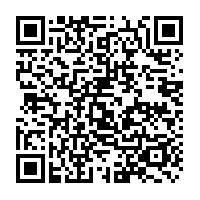
\includegraphics[width=0.375\textwidth]{imgs/QRcode.png}
   \caption{QR code per la richiesta di pagamento in BTC}
\end{figure}
Una volta generata la transazione di 0.0150 BTC verso il nagozio di Bob, Alice sempre attraverso il suo smartphone autorizza la transazione. Nel giro di pochi secondi Bob vedr\`a la transazione sul registro, e la transazione sar\`a quindi completata.
Possiamo esaminare la transazione effettuata una volta che \`e stata inclusa all'interno della blockchain usando un sito di \textit{explorer} (si veda~\cite{antonopoulos2017mastering} pp. 16-17).



